\documentclass{sig-alternate}
\usepackage{epstopdf}

\begin{document}

%TODO: cambiar este título horrible
\title{L'Ecuyer y velocidad WARP}

\numberofauthors{2}

\author{
    \alignauthor
    Gomez Vidal, Maximiliano\\
    \email{dgomezvi@alu.itba.edu.ar} \\
    \ \\
    Abramowicz, Pablo\\
    \email{pabramow@alu.itba.edu.ar} \\
    \ \\
    \alignauthor
    Sessa, Carlos\\
    \email{csessa@alu.itba.edu.ar} \\
    \ \\
    Villa Fern\'{a}ndez, Santiago\\
    \email{svillafe@alu.itba.edu.ar}
}

\maketitle

\begin{abstract}
En este art\'{i}culo se analiza el generador de n\'{u}meros pseudo-aleatorios
sugerido por L'Ecuyer y se lo pone a prueba utilizando el test de 
Kolmogorov-Smirnov y el test $\chi^{2}$. Se realiza tambi\'{e}n una simulaci\'{o}n
del tiempo de vuelo de una nave espacial mediante el m\'{e}todo de Montecarlo.
\end{abstract}

\keywords{L'Ecuyer, generador lineal congruencial, simulaci\'{o}n de Montecarlo,
 test $\chi^{2}$, test Kolmogorov-Smirnov, propulsi\'{o}n WARP}

\section{Introducci\'{o}n}\label{introduccion}

El concepto de aleatoriedad est\'{a} presente en diversos campos de la ciencia,
tales como la criptograf\'{i}a y la estad\'{i}stica.

En determinadas ocasiones es deseable generar secuencias de n\'{u}meros
aleatorios. Resulta l\'{o}gico pensar en generar dichas secuencias utilizando
una computadora. Sin embargo, los n\'{u}meros al azar surgen \'{u}nicamente
de procesos naturales que no pueden ser recreados en un dispositivo determinista
como lo es una computadora. La soluci\'{o}n a este problema consiste en utilizar
algoritmos que permitan generar secuencias suficientemente largas de n\'{u}meros
que presenten una distribuci\'{o}n estad\'{i}stica regular. Es decir, que no debe
ser posible distinguir mediante pruebas estad\'{i}sticas que la secuencia no
ha sido construida realmente al azar.

Uno de los generadores m\'{a}s conocidos de n\'{u}meros pseudo-aleatorios es
el generador lineal congruencial (LCG). 

En la secci\'{o}n \ref{generador} se 
analiza el generador de L'Ecuyer, que utiliza dos LCG para generar las secuencias.
En la secci\'{o}n \ref{pruebagenerador} se somete al generador de L'Ecuyer
a tests estad\'{i}sticos para analizar la distribuci\'{o}n de los n\'{u}meros
generados. En la secci\'{o}n \ref{triangular} se obtiene una distribuci\'{o}n
triangular a partir de la salida del generador. En la secci\'{o}n
\ref{simulacionpropulsor} se realiza una simulaci\'{o}n del tiempo de vuelo
de la nave USS Enterprise utilizando el m\'{e}todo de Montecarlo. Finalmente,
se exponen las conclusiones en la secci\'{o}n \ref{conclusiones}.

\section{Generador de L'Ecuyer}\label{generador}

El generador sugerido por L'Ecuyer combina dos LCG de acuerdo al siguiente 
algoritmo:

\textit{PASO 1}
Seleccionar una semilla $X_{1,0}$ en el rango $[1, 2147483562]$ para el LCG$1$
y $X_{2,0}$ en el rango $[1, 2147483398]$ para el LCG$2$.

\textit{PASO 2}
Evaluar cada generador individual

\begin{equation}
\label{LCG1}
X_{1,n+1} = 40014 \ X_{1,n} \ mod \ 2147483563
\end{equation}

\begin{equation}
\label{LCG2}
X_{2,n+1} = 40692 \ X_{2,n} \ mod \ 2147483399
\end{equation}

\textit{PASO 3}
Computar

\begin{equation}
\label{xn}
X_{n+1} = (X_{1,n+1} - X_{2,n+1}) \ mod \ 2147483562
\end{equation}

\textit{PASO 4}
Computar

\begin{equation}
\label{un}
U_{n+1} = 
    \begin{cases}
    \frac{X_{n+1}}{2147483563}, X_{n+1} > 0\\
     \ \\
    \frac{2147483562}{2147483563}, X_{n+1} = 0\\
    \end{cases}
\end{equation}

\textit{PASO 5}
Hacer $n = n + 1$ e ir al \textit{PASO 2}.

\section{Probando el generador de L'Ecuyer}\label{pruebagenerador}

Resulta de inter\'{e}s estudiar si la secuencia generada se encuentra
distribuida de manera uniforme. A continuaci\'{o}n se somete a prueba el
generador de L'Ecuyer utilizando el test $\chi^{2}$ y el test de 
Kolmogorov-Smirnov.

\subsection{Test $\chi^{2}$}\label{testchicuadrado}

Se desea establecer si es posible aceptar la hip\'{o}tesis $H_{0}:$ la secuencia
generada utilizando el algoritmo de la secci\'{o}n \ref{generador} corresponde 
a muestras de una variable uniforme $\mathcal{U}[0,1)$,
con un nivel de confianza del $95\%$. Para esto se generan $10,000$ n\'{u}meros 
utilizando $(0,2)$ como semillas. Luego se agrupan en $100$ intervalos de clase.

La media esperada en cada intervalo de clase es $E_{i} = 100$, pues se analiza 
una distribuci\'{o}n uniforme. El estad\'{i}stico dado por la ecuaci\'{o}n:

\begin{equation}\label{estadistico}
\chi^{2}_{0} = \sum_{i=1}^{100} \frac{(O_{i} - E_{i})^{2}}{E_{i}}
\end{equation}

resulta aproximadamente $98.84$.
Se observa que la distribuci\'{o}n $\chi^{2}$ subyacente posee $99$ grados de
libertad, puesto que se han considerado $100$ categor\'{i}as para agrupar los
n\'{u}meros generados.

Para el nivel de significaci\'{o}n deseado, $\alpha = 0.05$, se obtiene el
valor cr\'{i}tico $\chi^{2}_{99,0.05} = 124.3421$. Como 
$\chi^{2}_{99,0.05} > \chi^{2}_{0}$ se acepta $H_{0}$ y se determina que
los n\'{u}meros est\'{a}n distribuidos de manera uniforme. En la figura
~\ref{fig:clases} se observa la distribuci\'{o}n de los $10,000$ n\'{u}meros para
cada clase. En las figuras ~\ref{fig:duplas} y ~\ref{fig:ternas} se observa que no es
posible detectar patrones en la distribuci\'{o}n de la secuencia generada, puesto
que la misma presenta una densidad uniforme.

\begin{figure*}[hp]
\centering
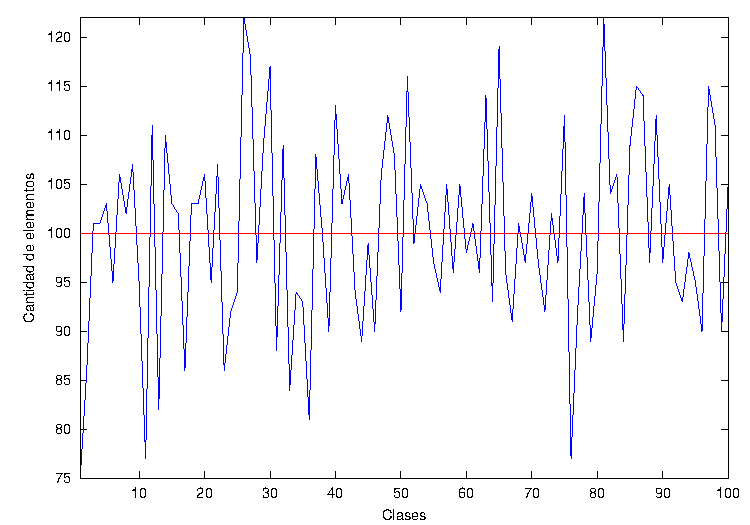
\includegraphics[scale=0.8]{graficos/clases}
\caption{Cantidad de resultados por categor\'{i}a para el test $\chi^{2}$}
\label{fig:clases}
\end{figure*}

\begin{figure*}[hp]
\centering
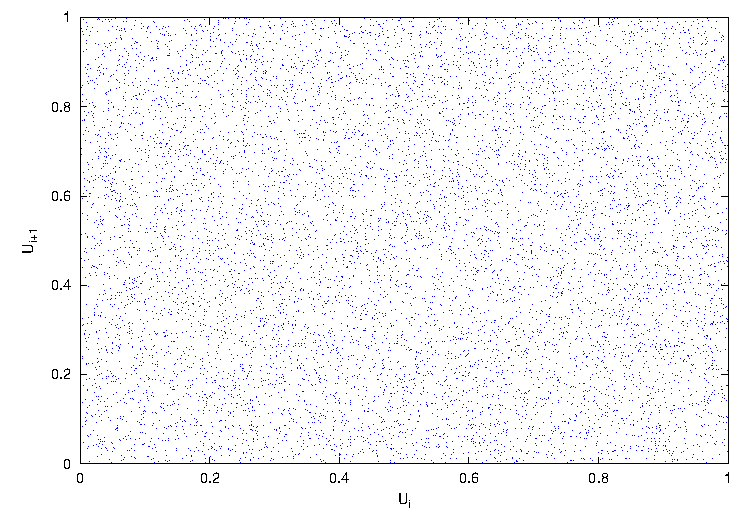
\includegraphics[scale=0.8]{graficos/duplas}
\caption{Duplas $(U_{i}, U_{i+1})$ de n\'{u}meros pseudo-aleatorios generados}
\label{fig:duplas}
\end{figure*}

\begin{figure*}[hp]
\centering
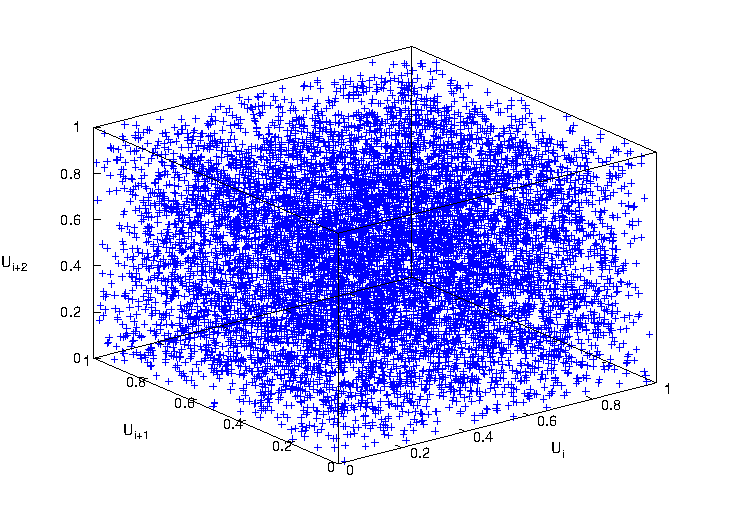
\includegraphics[scale=0.8]{graficos/ternas}
\caption{Ternas $(U_{i}, U_{i+1}, U_{i+2})$ de n\'{u}meros pseudo-aleatorios
generados}
\label{fig:ternas}
\end{figure*}

\subsection{Test Kolmogorov-Smirnov}\label{testks}

Este test se utiliza para contrastar uniformidad. Compara la distribuci\'{o}n
emp\'{i}rica obtenida a partir de una muestra con la distribuci\'{o}n te\'{o}rica
correspondiente a la variable aleatoria en estudio.

Se mantienen los mismos $10,000$ n\'{u}meros generados en la secci\'{o}n
\ref{testchicuadrado} y la misma hip\'{o}tesis $H_{0}$. Se realiza el test
correspondiente comparando la secuencia arrojada por el generador de L'Ecuyer
con otra muestra que presenta una distribuci\'{o}n uniforme. El resultado
arrojado es una aceptaci\'{o}n de $H_{0}$ con aproximadamente un $96.45\%$
de confianza, por lo que no se rechaza la hip\'{o}tesis nula a un nivel de 
significaci\'{o}n de 0.05. Es decir, la secuencia generada presenta una 
distribuci\'{o}n uniforme.

\section{Densidad triangular}\label{triangular}

%TODO
\section{Sistema de propulsi\'{o}n WARP}\label{simulacionpropulsor}

%TODO
\section{Conclusiones}\label{conclusiones}

\end{document}
